\section{Proposal's context, positioning and objectives}
\label{sec:context}

\subsection{Objectives and scientific hypotheses}
\label{sec:goals}

\Comments{Present the objectives and the research hypotheses ; present the scientific and technical barriers to be lifted ; present the expected results; if applicable describe any final products developed.}

\noindent\textbf{Context.}
In numerous fields of application, such as material sciences
or medical imaging, non-invasive acquisition devices such as magnetic
resonance, X-ray tomography or micro-tomography are required for
observation, measurements or diagnostic aids
(\eg \cite{Hildebrand1999,dcoeurjo_flin_ImPro}). %,dardenne2009variational}).
These acquisition devices usually generate volumic data, \ie
3D images, composed of regularly spaced data in a cuboidal domain.
3D volumes come from the segmentation of such 3D images.
They are also generated in scientific modelling because
numerous simulation schemes rely on the regularity of the data support
(\eg \cite{wojtan2007animating,jones2010directable,marechal2010heat}) and they are also the support inside 3D printing process.

%% TRIS: je crois avoir garder l'esprit, mais j'ai reformule pour
%% pour éviter les répétition et mieux coller avec le reste

%% Thanks to non-invasive acquisition devices such as magnetic
%% resonance, X-ray tomography or micro-tomography, processing
%% subsets or partitions in 3D  binary volumes is crucial in
%% numerous fields of application, such as material sciences
%% or medical imaging (\eg \cite{Hildebrand1999,dcoeurjo_flin_ImPro,dardenne2009variational}).
%% Many volumetric acquisition devices generate regularly spaced
%% data and we have to process the geometry of regions defined as subsets in these
%%   3-D images.}  \dav{Alternatively, modeling mathematical objects or
%%   complex natural phenomena on voxel grids often lead to efficient
%%   solutions
%%   \cite{wojtan2007animating,jones2010directable,marechal2010heat}):
%%   one can exploit the regularity of the grid as a support for the
%%   numerical simulation schemes, or us the grid as an efficient
%%   datastructure to represent complex geometrical objects \cite{kampe2013sg,Villanueva:2016:SSS:2856400.2856420,JaspeVillanueva2017SSVDAG}.}

%% \dav{\sout{3D \dav{binary} volumes come from the segmentation of magnetic resonance, X-ray tomographic or micro-tomographic images. 
%% They are also generated in scientific modelling and by voxel
%% editors. }}


PARADIS is a project about geometry of volume boundaries,
called \emph{digital surfaces} (fig.~\ref{fig:snow}). 
Keeping the digital nature of the data is an advantage
to do integer-only and exact computations,
to perform constructive solid geometry operations,
or to use efficient spatial data structures
(\eg \cite{kampe2013sg,Villanueva:2016:SSS:2856400.2856420,JaspeVillanueva2017SSVDAG}).
A drawback is its poor geometry, because a digital surface is only 
made up of quadrangular surface element (\emph{surfel} for short) 
whose normal vector is parallel to one axis whatever the resolution. 
Many tasks in computer graphics, vision and 3D image analysis require a richer geometry: 
rendering, surface deformation for simulation or tracking, precise geometric measurements, etc.
To perform relevant geometric tasks and 
to benefit from the above-mentioned advantages in the same time, 
we need to enhance the geometry of digital surfaces by estimating extra data for each surfel. 
\textbf{This project focuses on estimations of local and first-order geometric quantities
such as normal vector direction.}

\begin{figure}[hb]
  \centering
%
%\subfloat[]{ 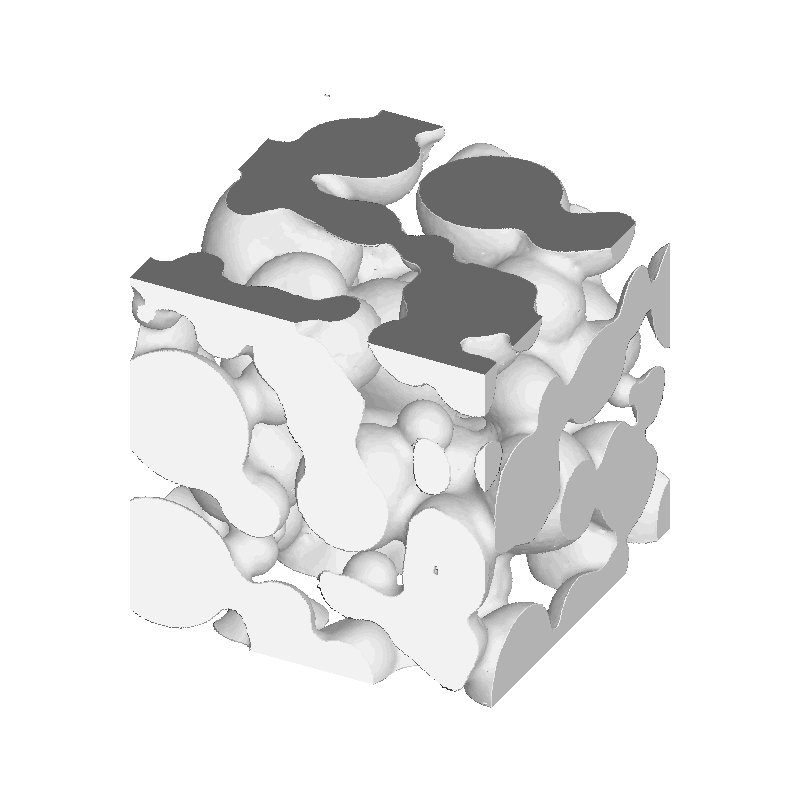
\includegraphics[height=0.2\textheight]{INH5_512_0}}
%
\subfloat[]{
\begin{tikzpicture}[spy using outlines={circle,yellow,magnification=2.5,size=2.8cm,connect spies}]
\node {\includegraphics[width=0.43\textwidth, trim= 0 0 10cm 0,clip=true ]{closeup-normals-3710x2112}};
\spy on (1.65,-0.2) in node [left] at (-0.95,-0.75);
\end{tikzpicture}
}
%
%
\subfloat[]{
\begin{tikzpicture}[spy using outlines={circle,yellow,magnification=2.5,size=2.8cm,connect spies}]
\node {\includegraphics[width=0.43\textwidth, trim= 0 0 10cm 0,clip=true ]{closeup-facets-3710x2112}};
\spy on (1.65,-0.2) in node [left] at (-0.95,-0.75);
\end{tikzpicture}
}
%
\caption{``ice-air'' interface in a micro-tomographic image of
  snow\protect\footnotemark. Local normal vectors are estimated
  at each corner (a) by computing relevant facets (b). This
  preliminary work does not extend the estimation to each surfel
  (see \sect{sec:estim:ds}). } 
\label{fig:snow} 
\end{figure}
\footnotetext{obtained by the 3SR Lab and CEN/CNRM - GAME URA 1357/M\'{e}t\'{e}o-France - CNRS, 
shared during ANR-11-BS02-009 DigitalSnow project.}

\noindent\textbf{Scientific bottleneck.}
The surface geometry within a patch around each surfel should be gathered to provide such estimations
-- \eg by polynomial fitting \cite{Cazals2005,Cazals2008}.
Almost all methods require at least one parameter that controls the size of the patch.  
On the contrary, this project aims at providing \emph{accurate} and \emph{parameter-free} estimators
based on a surface patch with \emph{adaptive} size.
Since we are looking for first-order estimations, the patch will be typically a piece of digital plane
that locally fits the digital surface. %(fig.~\ref{sub:pattern}).
A challenge is to cover the whole digital surface by maximal pieces of digital plane. 
Such a cover will not only provide a normal vector field, but will also provide, if computed
for several subsampled versions of the input 3D volume, a way of determining the scale 
at which noise is unlikely: a high number of very small digital plane segments indicate noise, whereas
smooth parts are decomposed into a smaller set of larger segments. Such a strategy was succefully proposed on 2d contours \cite{Kerautret2012}.

Contrary to the 2D case, what is challenging is that there is a combinatorial explosion
of maximal pieces of digital plane \cite{Sivignon2009} and that among them,
not all are tangent to the digital surface \cite{Charrier2011}.  
An opportunity to make a breakthrough regarding this issue is to consider the recent development
of \emph{plane-probing} algorithms \cite{LPRTCS2016, LPRDGCI2016, LPRJMIV2017},
proposed by the principal investigator and his collaborators.
These algorithms allow to decide
on-the-fly how to probe the digital surface and make grow a digital plane segment,
which is tangent by construction. The growth direction is given by both arithmetic and geometric properties.

\noindent\textbf{Objectives and expected results.}
PARADIS aims at analyzing digital surfaces with the help of plane-probing algorithms. 
Three distinct goals can be highlighted:
\begin{enumerate}[label=(G\arabic*)]
  \item %[(G1)]
The first one is to study extra arithmetic and combinatorial properties
of plane-probing algorithms. We expect to design an ultimate plane-probing algorithm that
only probes a part of digital surface \emph{as small as possible} to provide a relevant facet.
A formal definition of what is meant by \emph{small} and a theoretical upper bound will be provided.
In addition, we expect to correctly process non-convex parts by generating an underlying
minimal and connected piece of digital plane.  \label{goalppa} 
 \item %[(G2)] 
The second goal is to derive \emph{efficient}, \emph{accurate} and \emph{parameter-free} estimators
of \emph{local} and \emph{first-order} geometric quantities: normal vector (and surfel area as a by-product),
distance to boundary, voxel coverage (fig.~\ref{fig:2D}). We expect to derive such estimators from
the above-mentionned plane-probing algorithm and provide a theoretical evaluation of their accuracy
with respect to resolution. \label{goalestim}  
%(WP2).
 \item %[(G3)] 
The third goal is to provide a method and a tool for an automatic and \emph{multiscale} analysis of digital surfaces,
based on the number or the size of the computed facets for several subsampled versions of the input 3D volume. 
We expect to develop a tool that provides, without any parameter, the scale at which noise is unlikely. Based on
this tool, we may add other features like a 3D normal estimator robust to noise, \ie able to ignore some of
the residual variation that does not represent underlying structure and allowning an adaptative estimation to noise level.  \label{goalscale}
%(WP3). 
\end{enumerate}

\begin{figure}[hbt]
  \centering
\subfloat[]{ 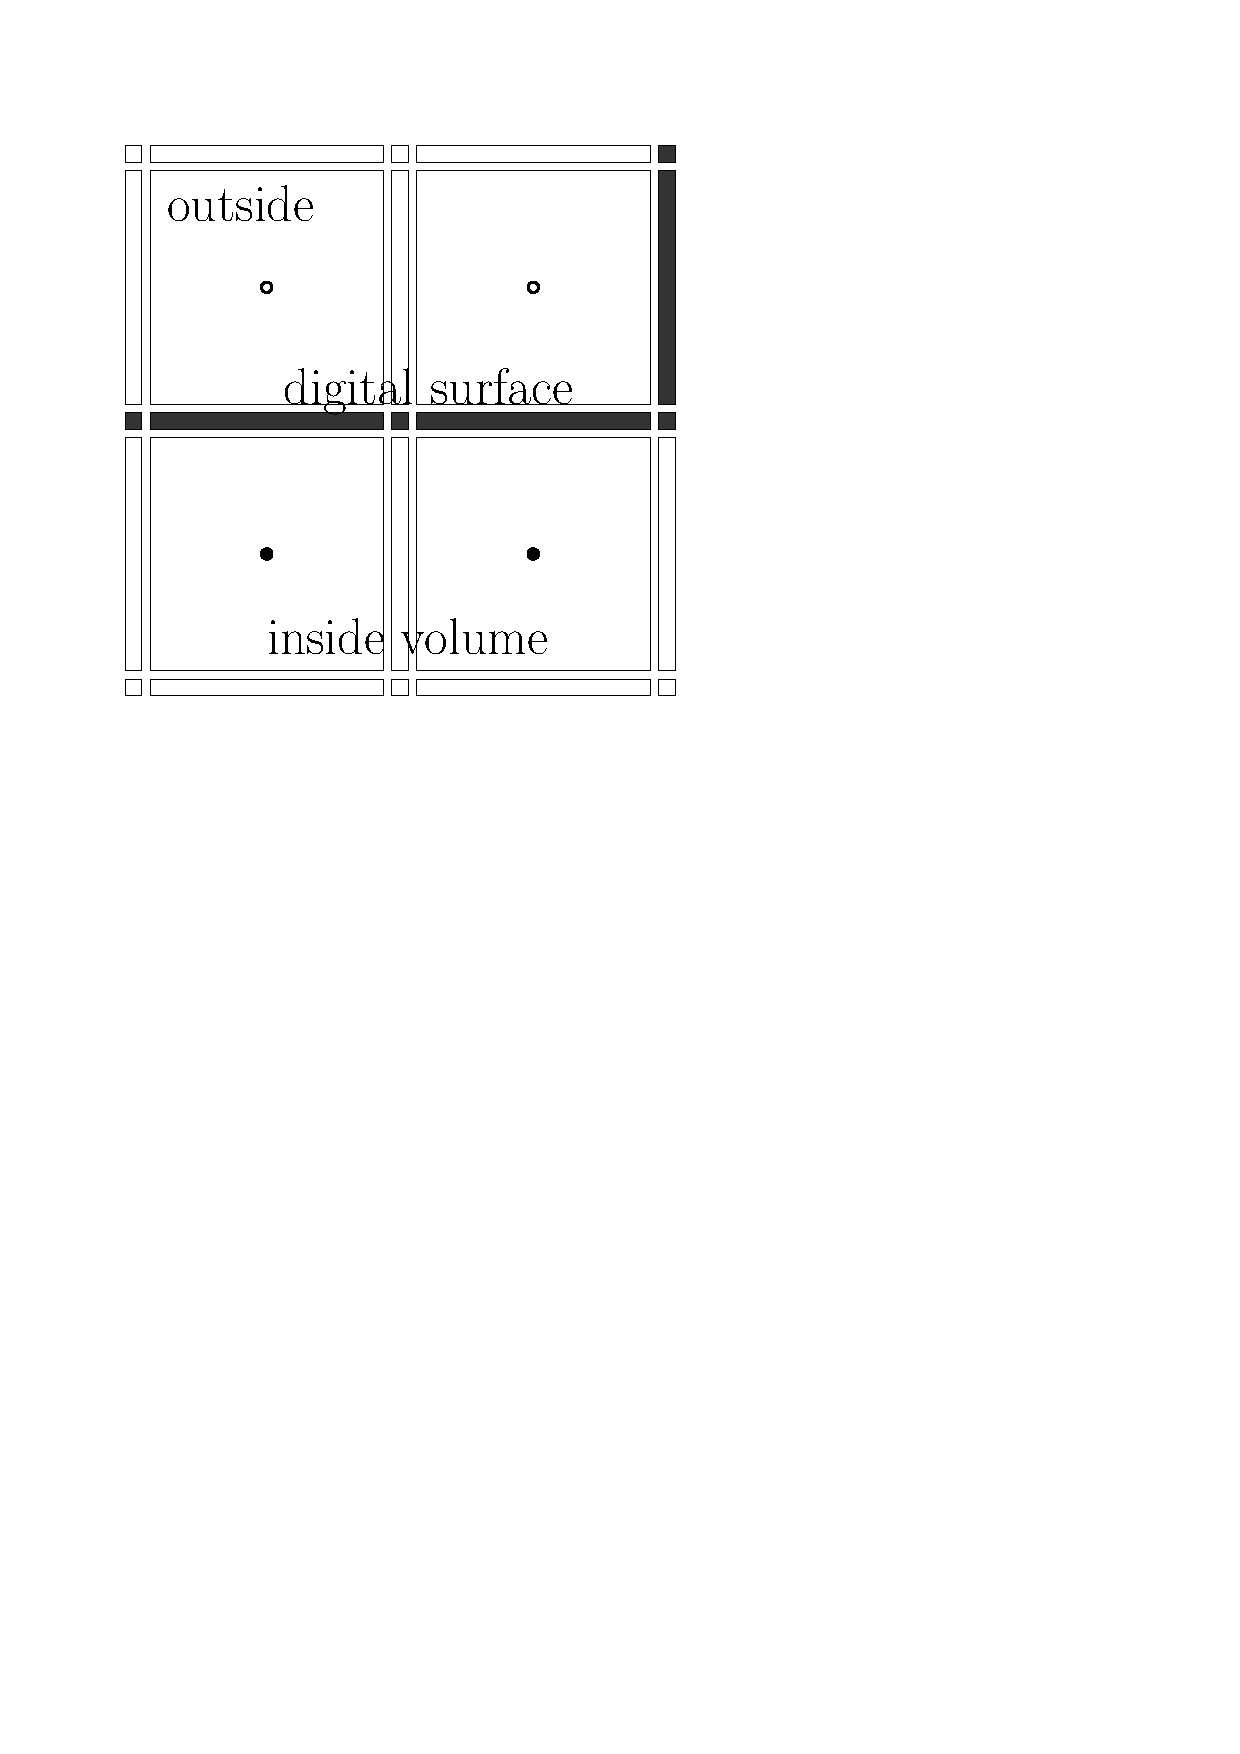
\includegraphics[width=0.13\textwidth,page=1]{square.pdf} } \hspace{0.05\textwidth}
\subfloat[]{ \includegraphics[width=0.13\textwidth,page=2]{square.pdf} } \hspace{0.05\textwidth}
\subfloat[]{ \includegraphics[width=0.13\textwidth,page=3]{square.pdf} } \hspace{0.05\textwidth}
\subfloat[]{ \includegraphics[width=0.13\textwidth,page=4]{square.pdf} } 
 \caption{2D illustration of a digital surface: voxels are big squares whose center is depicted by a black (resp. white) disk if it lies inside (resp. outside) the volume; surfels are elongated dark rectangles. We want to estimate a relevant normal vector at a given surfel (b), but also to locally reconstruct a boundary perpendicular to this normal vector in order to derive distance and coverage estimations (c-d).} 
\label{fig:2D} 
\end{figure}

New algorithms, theoretical results and experimental studies will be disseminated through papers submitted to
top venues or in peer-reviewed international journals. Plane-probing algorithms and derived estimators
will be implemented in the open-source C++ library {\DGtal}, whereas the tool will be added to {\DGtalTools},
a companion project of {\DGtal}, with an {\IPOL} paper for coding details.  

%sqdf \ref{goalppa} qsdf \ref{goalestim}, \ref{goalscale}. 
 
 %1-WP0: algorithm purely local, from any starting point, which leads to a reduced basis and retrieves any normal
%1-WP1: pattern generation: minimal number of tiles, connected, 
%2-WP2: estimateur + ordre de convergence theorique + applis ?
%3-WP3: outils qui prend un volume et sors un sous-échantillon non bruité, ou un ensemble de voxels à différentes tailles (publi IPOL)
%=> for each publication and implementation in DGtal. 

%transition not relevant here
%Since there are so many perspectives and paths to follow, this project needs to strengthen a team of experts by full-time workers in order to make the best of them. 

\subsection{Originality and relevance in relation to the state of the art}
\label{sec:art}

\Comments{Emphasise the ambitious nature of the proposal and the novelty of the research in relation to the state of the art ; show the possible contributions of project partners to the state of the art ; present any preliminary results. In the case of a project proposal following up on previous project(s) already funded by ANR or by another body, provide a summary of the results achieved and clearly describe the new issues raised and the new objectives set out in the light of the earlier project.}

In each of the three following sections, we describe the state of the art and explain the originality and relevance of our project.
%In this section, we underline the novelty of the proposed approach in relation to the state of the art.  
We focus on the estimation of the normal direction, which is the most challenging task with the biggest impact. 
Other first-order quantities are either obtained as a by-product of the normal estimation (\eg surfel area \cite{Lachaud2016})
or carry position information already approximated by the digital surface itself (\eg distance to boundary).

In addition, a digital surface is a quadrangular mesh. The vertex set consists of evenly spaced data points
whose coordinates are (half-)integer. This specific point cloud approximates a continuous 2-manifold under a
uniform noise model due to discretization errors. That is why, we review the most common methods for normal estimation
not only on digital surfaces, but also on meshes and point clouds.
%TODO nombreuses applications de normal estimation ce qui explique qu'il y ait beaucoup de travaux.  

%% Note that we do not present 2D estimators (\eg \cite{Provot2011,Esbelin2011,Esbelin2016}),
%% with the exception of \cite{Lachaud2007}, which is parameter-free and used in 3d estimators
%% \cite{Lenoir1996,Tellier1999,Lachaud2003}. 

%% \todo[inline]{Sébastien dit: L'utilisation de l'expression "state of the art"
%% est incorrecte dans le paragraphe suivant et pourrait laisser croire qu'on n'a
%% pas compris la question. Le
%% \url{https://en.wikipedia.org/wiki/State_of_the_art}, c'est ce qui se fait de
%% mieux dans la littérature par rapport à ce que nous on regarde. Ceci dit, la
%% première phrase plus haut ("In this section...") est correcte. Mais, ensuite,
%% on parle que ce ce que nous proposons, possiblement pas assez de ce qui se fait
%% deja dans le domaine pour resoudre ce genre de question et en quoi on est
%% different/mieux. Je crois que ce serait bien ici d'annoncer les sections 1.2.1,
%% 1.2.2 et 1.2.3 et mentionner qu'elles répondent bien à ce qui est attendu: "In each of the three following sections, we describe the state of the art and explain the originality and relevance of our project."}
%%TRIS: OK je crois avoir corriger en fonction de ce que tu dis

Since one of the goals of the project is to propose an accurate and parameter-free normal estimator,
we focus on user-defined parameters and we check if the estimator preserves sharp features and,
for digital surfaces only, is \emph{multigrid-convergent}, \ie the smaller the grid step,
the higher the resolution, the more accurate the estimator (fig.~\ref{fig:multi}). 

\begin{figure}[htbp]
  \centering
  \subfloat[$h=0.8$]{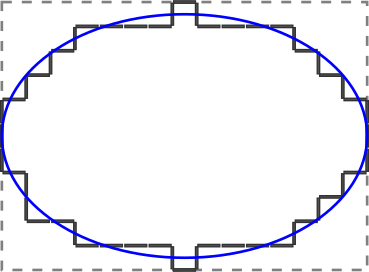
\includegraphics[width=0.25\textwidth]{conv08}}\hspace{0.05\textwidth}
  \subfloat[$h=0.5$]{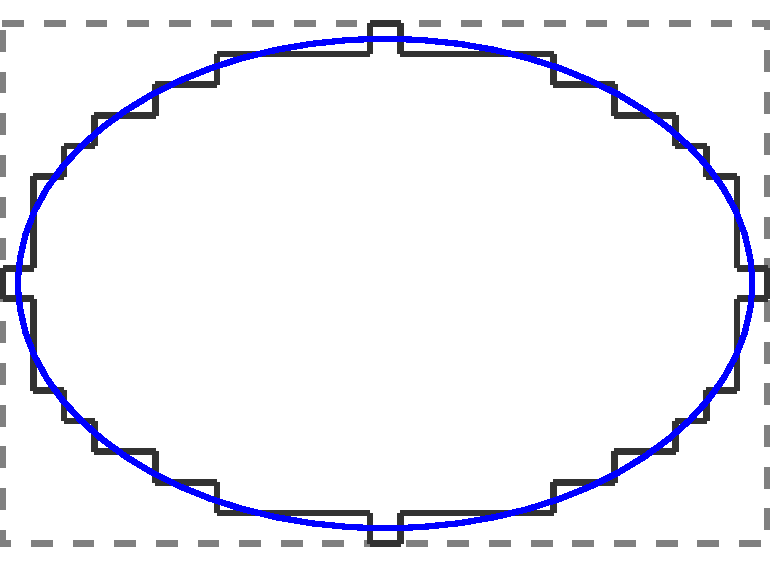
\includegraphics[width=0.25\textwidth]{conv05}}\hspace{0.05\textwidth}
  \subfloat[$h=0.2$]{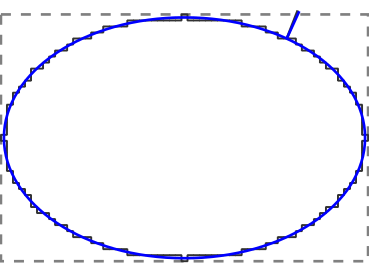
\includegraphics[width=0.25\textwidth]{conv02}}
  %% \subfloat[]{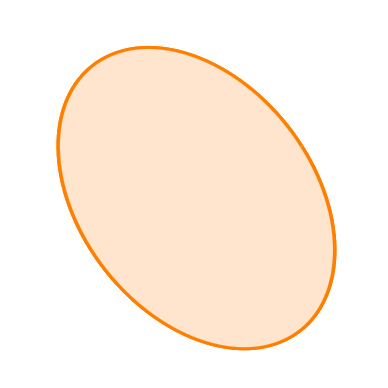
\includegraphics[width=3.5cm]{multi-ellipse-0}}
  %% \subfloat[]{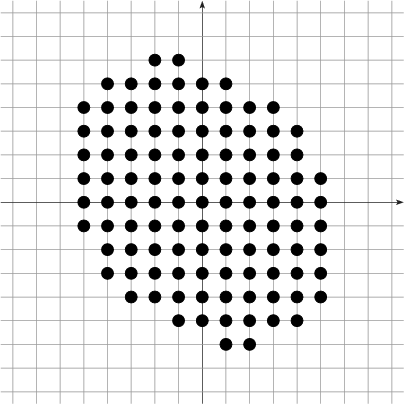
\includegraphics[width=3.5cm]{multi-ellipse-1}}
  %% \subfloat[]{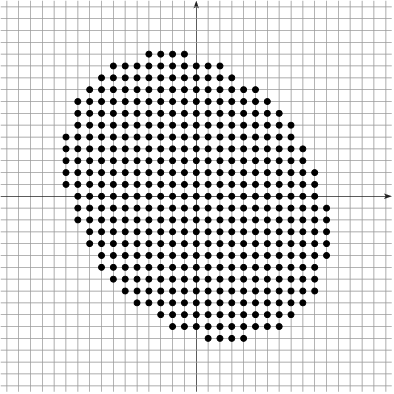
\includegraphics[width=3.5cm]{multi-ellipse-2}}
  %% \subfloat[]{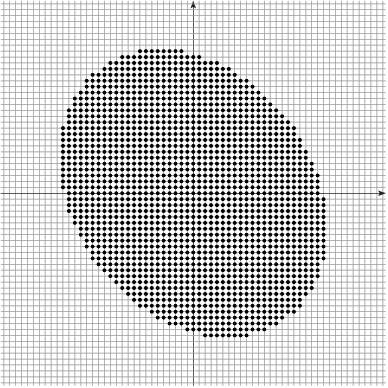
\includegraphics[width=3.5cm]{multi-ellipse-4}}
  \caption{Digitization of a 2D ellipse at a grid step $h$ taking decreasing values.
    A multigrid-convergent estimator is such that the estimated quantity at a point of a
    digital curve or surface gets closer to the one of the underlying continuous shape
    at a close enough point as $h$ tends to zero.
    %%TRIS je supprime car j'ai le sentiment que cette remarque apporte plus de questions que de réponses 
  %% Note that the length of the digital
  %%   contour \dav{(length defined for instance as its number of
  %%     surfels) does not tend to the perimeter of the underlying
  %%     ellipse as $h$ decreases.}
  }
  \label{fig:multi}
\end{figure}


%% \noindent\textbf{Digital surface and multigrid convergence.}

%% 3D volumes are collections of cubes. % of size $h$, called \emph{grid step}. 
%% Their topological boundary is a quadrangular mesh called \emph{digital surface}.
%% The vertex set consists of evenly spaced data points whose coordinates are
%% half-integer. This set approximates a continuous 2-manifold under a uniform
%% noise model. 
%% %TODO: Lachaud Thibert

%% Most of the time, when we are working with a digital surface, we are 
%% interested in the geometry of a continuous shape whose digitization
%% is the input 3D volume.
%% Formally, given a compact shape $X \subset \R^3$,
%% its digitization at grid step $h \in \R^+$ is $\Dig(X) := \{z \in \Z^3, hz \in X\}$.
%% If we denote the axis-aligned closed cube centered on $z \in h\Z^3$ and of size $h$ as $Q_z^h$,
%% the cube embedding of a digital set $Z$ at grid step $h$ is $\underset{z\in Z}{\cup}Q_z^h$.
%% Let $\partial_h X$ be the topological boundary of the embedding of the digitization of $X$: 
%% \[
%% \partial_h M := \partial \Big( \underset{z\in\Dig(X)}{\bigcup}Q_z^h \Big).
%% \]

%% We expect that a given geometric quantity, such as a normal vector,
%% computed at a point of a digital surface ($\partial_h X$),
%% is close to the one of the underlying continuous shape ($X$) at a close enough point. 

%% \begin{Definition}[multigrid-convergent estimator \cite{Coeurjolly2012}]
%%   \label{def:multigrid-convergence2}
%%   The estimator $\hat{Q}$ is {\em multigrid-convergent} for the family
%%   {\Shapes} if and only if, for any shape $X \in \Shapes$,
%%   there exists a grid step $h_X>0$ such that the estimate
%%     $\hat{Q}(\Dig(X),y,h)$ is defined for all
%%   $y \in \partial_h X$ with $0<h < h_X$, and for any $x \in \BT{X}$,
%%   \begin{equation*}
%%     \forall y \in \partial_h X \text{~with~} \| y - x \|_1 \le h, \quad
%%     \hat{Q}(\Dig(X),y,h) - Q(X,x) | \le \tau_{X,x}(h),
%%   \end{equation*}
%%   where $\tau_{X,x}: \R^{+*} \rightarrow \R^+$ has null limit at
%%   $0$.
%%   %% This function defines the speed of convergence of $\hat{Q}$
%%   %% toward $Q$ at point $x$ of $\BT{X}$. The convergence is {\em uniform} for
%%   %% $X$ when every $\tau_{X,x}$ is bounded from above by a function
%%   %% $\tau_X$ independent of $x \in \BT{X}$ with null limit at $0$.
%% \end{Definition}

%% The accuracy of a multigrid-convergent estimator depends on the grid step:
%% the smaller the grid step, the more accurate the estimator. 

\subsubsection{Normal estimation on point clouds, meshes and digital surfaces}
\label{sec:estim:all}

%%tenses
%%present rapporter ce qu'un auteur pense, ecrit, fait generaux
%%past ce qu'un auteur a fait, trouve
%%present perfect ce qui se fait dans une communaute
%%http://ueberfachliche-kompetenzen.ethz.ch/dopraedi/pdfs/Mayer/guidelines_review_article.pdf

%interet des normales
Numerous tasks rely on the quality of normal estimation in point clouds, such as
surface reconstruction, scene understanding or point-based rendering to name a few.
In surface fairing or mesh denoising, a common approach is to first compute a relevant
normal field and then evolve the mesh to match the smoothed normals.
Hence, a lot of normal estimation methods have been proposed. 

\noindent\textbf{Fitting.}
\citeauthor*{Hoppe1992} \cite{Hoppe1992} estimated the normal at a given data point by computing
the least squares best fitting plane to a point set within a neighborhood
around the point of interest.
Other fitting surfaces have also been used, such as jets, \ie truncated Taylor expansion
of a surface expression \cite{Cazals2005,Cazals2008}. 
All fitting methods first consist in collecting the points used for the fitting.
In the mesh case, a breadth-first search visits the neighbors until enough points
have been collected. In the point-cloud case, one typically resorts to the k-nearest-neighbors
strategy. In both cases, the number of points to collect is usually a user-defined parameter,
even if some heuristics have been proposed to select it automatically \cite{Hoppe1992,Cazals2005}.
All fitting methods tend to smooth sharp features, and thus fail to correctly estimate normals
near edges.  

%%TRIS ok j'ai pris en compte cette remarque (cf. debut de section pour la convention utilisee)
%% \todo[inline]{"first use", "propose", "propose", "has been proposed": Choisir si on parle de la littérature au passé ou au présent et être cohérent. (Perso, je prefere le passe).}



\noindent\textbf{Voronoi diagram.}
Instead of approximating the tangent space, another familly of methods is based on the
Voronoi diagram to estimate at best the orthogonal space. \citeauthor*{Amenta1999} \cite{Amenta1999}
first used the furthest vertex of the Voronoi cell to estimate the normals of point clouds.
In order to get more stable estimates, \citeauthor*{Alliez2007} \cite{Alliez2007} proposed to apply linear fitting
to the Voronoi cell or to the union of Voronoi cells into a neighborhood. 
\citeauthor*{Merigot2011} \cite{Merigot2011} proposed an improvement %, called Voronoi Covariance Measure (VCM),
by taking a weighted average of covariance matrices of Voronoi cells instead of
taking the covariance matrix of their union. In their method,
only the intersection between the Voronoi diagram and a ball around the data point
is taken into account in order to get purely local information about the surface geometry.
A digital variant was proposed by \citeauthor*{Cuel2015} \cite{Cuel2015}. 

\noindent\textbf{Integral invariants.}
In the mesh case, another method sums up the surface geometry within a ball by 
computing integrals over the intersection between the ball and the volume
bounded by the mesh \cite{Pottmann2009}. The covariance matrix of the intersection set 
provides a way to estimate principal curvatures, principal directions and normal direction.
A digital variant was proposed by \citeauthor*{Lachaud2017} \cite{Lachaud2017}.
%
Note that the ball radius is a user-defined parameter in these
methods. In addition, the ball radius is usually the same for
the whole digital surface and completely ignores the features.
The above-mentionned digital variants \cite{Cuel2015,Lachaud2017}
are multigrid-convergent for digitization of smooth shapes if
the radius is conveniently chosen with respect to
the grid step.
%% TRIS: je trouve cet ajout poins pertinent (curvature estimator) et redondant avec la suite
%% \dav{In dimension 2, multigrid convergent
%%   parameter-free integral invariant curvature estimators can be
%%   derived \cite{Coeurjolly2014IIfree} but  extension to 3-D surfaces
%%   is not trivial (see below).}
%setting the ball radius from the
%  digital object boundary characteristics. Heuristics have been given
%  in 3-D but it is still an open problem whether multigrid convergent
%  and parameter-free curvature or normal vector estimators exist in 3-D.}

\noindent\textbf{Convolution.}
Starting from raw normal vector estimations (\eg unit
vectors perpendicular to surfels), several approaches refine the
estimation by convoluting the raw normals using a given smoothing
kernel. This technique has been proposed on digital curves
\cite{Esbelin2011,Esbelin2016} and surfaces
\cite{papierthese,Fourey2009} with the following drawbacks:
the user must specify the kernel parameters, including its size,
and the treatement, which is usually isotropic, smoothes out
sharp features. However, if the kernel size is some function of the
grid step, multigrid convergence can be obtained in 2D \cite{Esbelin2011}.
In mesh denoising, more advanced local filters, such as the bilateral one,
are used to preserve sharp edges and corners, but several parameters
are user-defined \cite{fleishman2003bilateral,zheng2011bilateral}.

\noindent\textbf{Variational approaches}. Another but similar approach
consists in minimizing a global energy function instead of applying a
local, iterative scheme. These techniques start from a raw estimation
of the normal vector field and use a complex variational scheme to obtain
a piecewise smooth regularization of the input field. The literature is
vast on this subject, see for instance \cite{zhang2015variational}. 
Applied to digital surfaces, a stable and piecewise smooth normal vector field
was obtained \cite{CoeurjollyFGL16} by a time-consuming algorithm and without
any guarantee of convergence. 

%% We conclude this
%%   overview by variational approaches aiming to denoise a surface or a
%%   normal vector field while preserving some features. Most techniques
%%   start from a raw (isotropic) estimation of the normal vector field
%%   and minimize an energy function to obtain a close piecewise smooth
%%   regularization of the input field. The literature is large on this
%%   subject, see \cite{CoeurjollyFGL16,zhang2015variational} for recent
%%   papers. These techniques can be seen as post-processes of a raw
%%   estimate and require complex schemes to solve the variational
%%   problem. Applied to digital surfaces, we obtain very robust and
%%   smooth normal vector field but the algorithm is time consuming and
%%   we are losing the pointwise multigrid convergence property.}

\noindent\textbf{Randomized Hough Transform.}
Finally, let us mention also probabilistic methods based on the Randomized Hough Transform.
Boulch and Marlet \cite{Boulch2012} considered many random triples of data points in a neighborhood
and bin their normal direction into a spherical histogram.
Maximal vote provides the normal estimate. However, their method has many input parameters,
the first of which is the size or radius of the neighborhood. 


\subsubsection{Parameter-free and adaptive normal estimators on digital surfaces}
\label{sec:estim:ds}

All reviewed methods have drawbacks. The few methods that perform an anisotropic
treatment to preserve features may be complex to implement, time-consuming, with
many user-defined parameters. The simplest methods have at least one parameter
that controls the size of the neighborhood for the whole data set and smooth out
sharp features.  

On the other hand, the specificity of digital surfaces makes the design of parameter-free
and adaptive estimators possible. The trick is to perform a uniform fitting of the data points by a plane.
In addition, instead of specifying the number of data points \emph{a priori}, they are added
step by step, while a maximal admissible error is not reached. This threshold is not a user-defined
parameter, but a known constant, because the data points follow a known uniform noise model
in case of digital surfaces. In 2D, methods based on digital straight segments (DSSs) follow
this approach.

The set of maximal DSSs, \ie inextensible straight parts, can be computed by one scan of the
digital curve \cite{Feschet1999,Feschet2005} and provides a multigrid-convergent
normal estimator \cite{Lachaud2007} (and normal integration over the digital curve yields
a multigrid-convergent length estimator \cite{Coeurjolly2004}). In addition to
convergence, this normal estimator has several sought-after properties:
it preserves sharp features (fig.~\ref{fig:corner}) and local convexity \cite{Roussillon2011},
without any input parameter. 
In addition, asymptotic properties of maximal DSSs can be used to estimate the local amount
of noise along the digital curve \cite{Kerautret2012}.  
\begin{figure}[htbp]
  \centering
  \subfloat[]{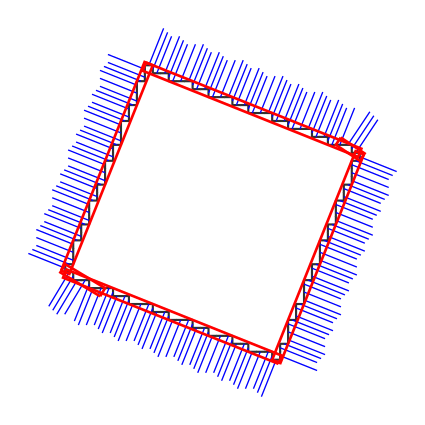
\includegraphics[width=0.28\textwidth]{square-g02-arith}}
  \subfloat[]{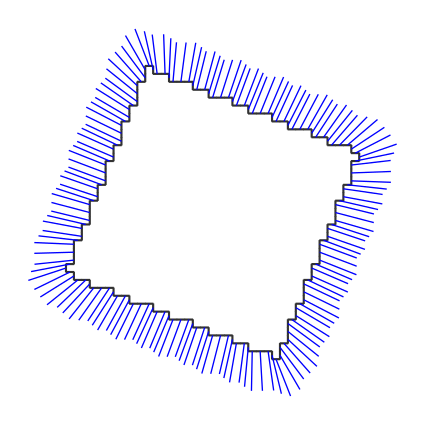
\includegraphics[width=0.28\textwidth]{square-g02-p50}}
  \subfloat[]{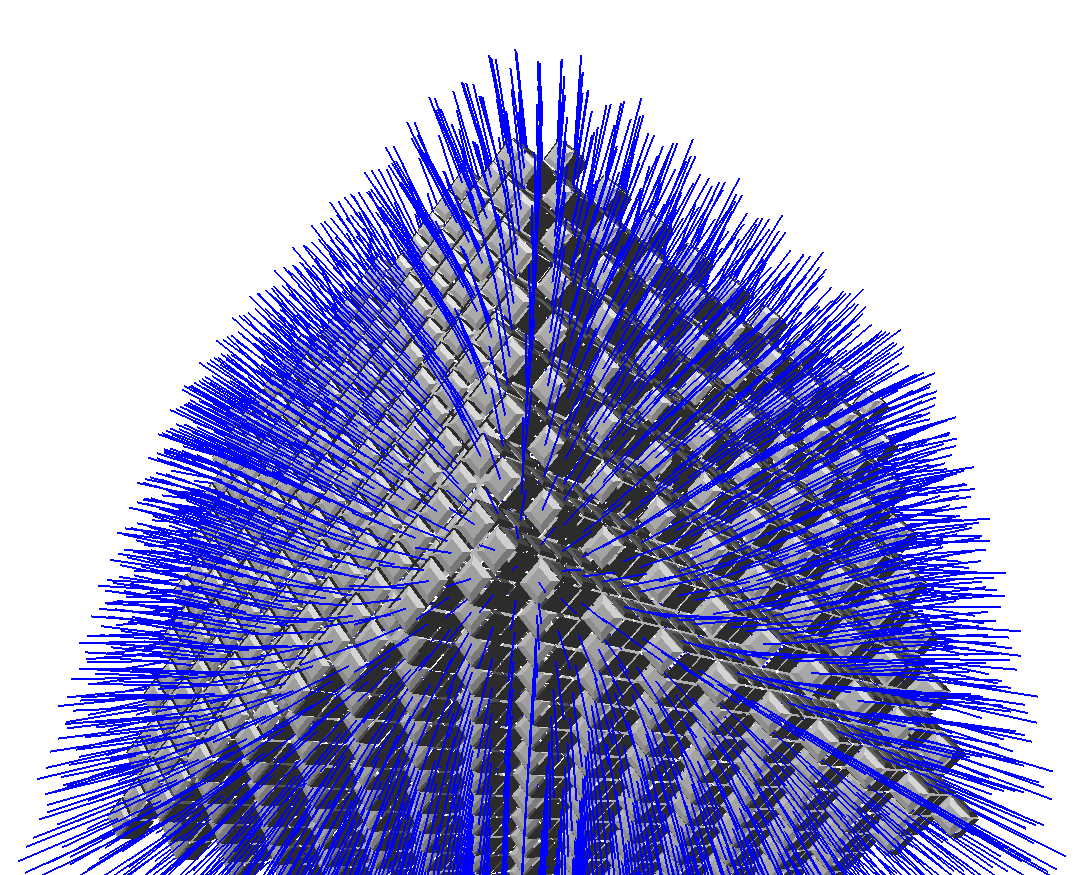
\includegraphics[width=0.3\textwidth]{cube}}
  \caption{Maximal DSSs provide multigrid-convergent normal estimates that preserves sharp features (a). 
    Almost all other methods, such as convolution of the raw normals, smooth them out as shown in (b) and (c).
    Finding a parameter-free, multigrid-convergent normal estimator that preserves sharp features is still a
    challenge in 3D.}
  \label{fig:corner}
\end{figure}

In higher dimension, to the best of our knowledge, only one parameter-free normal estimator
has been proposed in 3D \cite{Lenoir1996,Tellier1999} and extended to nD \cite{Lachaud2003}.
It is based on maximal DSSs on 2D slices. Maximal DSSs provide windows of adaptive size
but the slicing truncates the geometric information and leads to
an artificial spatial variability because two neighbor surfels only
share one slice over two. 

Given an estimator with an input size parameter, a general strategy to automatically and adaptively select
the parameter value consists in considering the size of maximal DSSs. 
The idea of such a hybrid method was first used in \cite{Devieilleville2009}
for a comparative study of 2D normal estimators and then in \cite{Coeurjolly2014IIfree}
for mean curvature estimation by integral invariants.
In 2D, this strategy is quite interesting for higher-order estimators such as curvature,
but is totally disproportionate for normal estimation since maximal DSSs straightforwardly give a good estimator. 
In 3D, even if this hybrid method may be useful for normal estimation, its computation cost may be rather high,
because we must take into account the preprocessing cost to approximate the parameter value for each surfel,
and the cost of the original estimator without any optimization trick that takes profit of the neighboring
computations with the same parameter value, as done in \cite{Lachaud2017}. 

Finally, another possible approach is to mimic the 2D tool box by computing the set of
digital plane segments (DPSs) that locally fits the digital surface. This approach
has been used for surface area estimation \cite{Klette2001}, reversible polyhedrisation
\cite{Sivignon2004} and normal estimation \cite{Charrier2011}. In the latter approach,
DPSs are initialized by a maximal circular neighborhood around a seed and then extended
without updating their normal vector. Even if it is a consistent definition of maximality,
this approach badly recovers the geometry of the digital surface near sharp edges and corners. 
The challenge is to find how to scan the digital surface to efficiently recognize DPSs
whose size and shape reveal the local geometry. 

\subsubsection{Digital plane segments: recognition and generation}
\label{sec:dps}

\noindent\textbf{Recognition of digital plane segments.}
A \emph{digital plane} is an infinite digital set that 
consists of several consecutive and parallel layers of coplanar points. 
It is defined by a (nonzero) normal $\vec{n} \in \Z^3$ and a position $\mu \in \Z$ as follows
\cite{reveilles1991}:  
\begin{equation}
  \label{eq:plane}
\Plane{\mu}{\vec{n}} := \{ \vec{x} \in \Z^3 \ | \ \mu \leq \vec{x} \cdot \vec{n} < \mu + \|\vec{n}\|_1 \}.
\end{equation}

Given a finite digital set $\Set$, the \emph{recognition problem} consists in providing
$\mu$ and $\vec{n}$ such that $\Set \subseteq \Plane{\mu}{\vec{n}}$ if they exist.
Note that such a recognition problem can have zero or infinitely many solutions.
One solution can be found in linear time, \ie in $O(|\Set|)$, by linear programming
and all solutions can be found in $O(|\Set|\log{(|\Set|)})$ by computational geometry tools.
See \cite{Brimkov2007} for a review on digital planarity.

However, one usually wants to add data points step by step and incrementally update the solution
or the set of solutions. In this on-line framework, optimal algorithms are difficult
to implement and are in all probability slow in practice due to a high constant in the asymptotic
upper bound (see for instance \cite{Buzer2003}).
On the other hand, there are fast geometrical algorithms but with higher theoretical bounds,
\eg \cite{Gerard2005, Charrier2008, Veelaert2012}.
%\cite{Gerard2009} preimage
%\cite{Stojmenovic1991} separation
%Provot2006, largeur

Actually, the main challenge is not really to recognize DPSs, but more to find which data points
should be taken into account during the recognition process to obtain DPSs tangent to the digital
surface. In addition, as noted in \cite{Charrier2011}, most inextensible digital planar sets are not
characteristics of the local geometry of the shape and finding the smallest subset which covers
the digital surface has been shown to be NP-complete \cite{Sivignon2009}.
Segmentation methods usually make a point set grow from a seed by a breadth-first search according
to some heuristics and decide whether the current set is a piece of digital plane or not
(see, for instance, \cite{Klette2001} or \cite{Sivignon2004}). 
%\cite{Provot2009} un peu different car parametre de bruit
The results are however highly dependent on the chosen heuristics.   

Until recently, artihmetic properties of digital planes have not helped so much.
Pionneering incremental recognition algorithms based on arithmetic properties
\cite{Debled1994,Mesmoudi2002} are neither as easy-to-implement nor as fast as
purely geometric ones, such as \cite{Gerard2005}.  
The work of V. Berth\'{e} and T. Fernique \cite{Fernique2009,Berthe2011}, 
based on multidimensional continued fractions and desubstitution on words,
is quite interesting from a theoretical point of view. However, their algorithm,
which reduces a piece of digital surface until no transformation is possible,
is not of practical interest because it requires the whole point set to be known
in advance and must be coupled with another recognition algorithm at the last step.  

\noindent\textbf{Preliminary results: plane-probing algorithms.}
A novel approach was proposed by the principal investigator and his collaborators
\cite{LPRTCS2016, LPRDGCI2016, LPRJMIV2017}. 
Given a digital plane $\Plane{\mu}{\vec{n}} \subset \Z^3$
and a starting point $\vec{p} \in \Set$, 
a \emph{plane-probing algorithm} computes the parameters of a digital plane $\Plane{\mu'}{\vec{n}'}$
containing $\vec{p}$ by sparsely probing $\Plane{\mu}{\vec{n}}$ with the predicate
``is $\vec{x}$ in $\Plane{\mu}{\vec{n}}$?''. The parameters of $\Plane{\mu}{\vec{n}}$
and $\Plane{\mu'}{\vec{n}'}$ are expected to be equal when the algorithm terminates.
%for any $\vec{p} \in \Plane{\mu}{\vec{n}}$. 

What makes plane-probing algorithms promising is that they decide on-the-fly how
to probe the digital surface and make grow a piece of digital plane, which is
tangent by construction. 
The first algorithm of this category has been proposed in \cite{LPRTCS2016}.
Its principle is to deform an initial unit tetrahedron set at the starting point
with only unimodular transformations. Each transformation is decided by looking
mostly at a few points around the tetrahedron. These points are chosen so that
the transformed tetrahedron lies in $\Plane{\mu}{\vec{n}}$, with the same volume,
but closer to the upper plane
$\UpperPlane{\mu}{\vec{n}} := \{ x \in \R^3 \ | \ x \cdot \vec{n} = \mu + \|\vec{n}\|_1 \}$.
At the end of this iterative process, one face of the tetrahedron has an extremal
position in the plane and is thus parallel to $\UpperPlane{\mu}{\vec{n}}$.

New plane-probing algorithms were proposed in \cite{LPRDGCI2016, LPRJMIV2017}. 
They also iteratively deform an initial tetrahedron and stop when one face is
parallel to $\UpperPlane{\mu}{\vec{n}}$ (see fig.~\ref{fig:ppa} for an illustration). 
%
\begin{figure}[htbp]
  \centering
  \subfloat[]{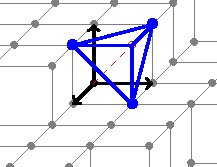
\includegraphics[width=0.17\textwidth]{triangle-1-2-5-0-0}}
  \subfloat[]{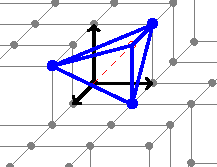
\includegraphics[width=0.17\textwidth]{triangle-1-2-5-0-2}}
  \subfloat[]{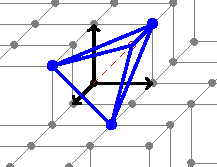
\includegraphics[width=0.17\textwidth]{triangle-1-2-5-0-4}}
  \subfloat[]{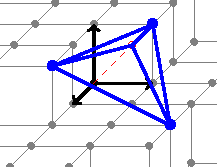
\includegraphics[width=0.17\textwidth]{triangle-1-2-5-0-6}}
  \subfloat[]{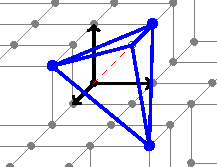
\includegraphics[width=0.17\textwidth]{triangle-1-2-5-0-8}}
  \caption{The current tetrahedron is depicted in blue. It is initialized at a corner (a) 
    and it is then deformed step by step by the \emph{R-algorithm} proposed in \cite{LPRJMIV2017} (b-e).
    When the algorithm terminates (e), the normal of the facet not incident to the fixed vertex
    is equal to the normal of the underlying digital plane, \ie $(1,2,5)$.}
    \label{fig:ppa}
\end{figure}
%
However, these new algorithms differ from the first work on several aspects.
First, they are simpler, because they repeat one simple operation instead
of several possible transformations depending on the current onfiguration
as in \cite{LPRTCS2016}.  
Second, one vertex of the evolving tetrahedron is a fixed point lying above the 
starting point and the opposite triangular facet (fig.~\ref{fig:ppa}). The position
of the evolving tetrahedron is thus better controlled than in \cite{LPRTCS2016}. 
Last, a geometric criterion is used so that the evolving tetrahedron is not
too much elongated during the computation.  

%surface
In addition, these algorithms are used for digital surface analysis in \cite{LPRJMIV2017}.
One drawback of this preliminary work is the processing of non-convex parts.
This case requires to associate a piece of digital plane to the tetrahedron.

\noindent\textbf{Discretization and generation.}
%generation de plans
Due to the analytical definition of digital plane, its topological and
arithmetical properties, one can efficiently generate an arbitrary piece
of digital plane using breadth-first traversal and incremental computations.
However, if the piece of digital plane is required to be projected into a
given polygon or simply a triangle as in \cite{LPRJMIV2017}, this approach
is not always possible, because acute angles can make the digital set disconnected. 

%discretisation de polygone en 3D
The standard analytical model provides a consistent way to discretize a $m$-simplex
in $n$D with topological guarentees, \ie into a $(n-1)$-connected, tunnel-free
and bubble-free point set \cite{Andres2003}. This model was successfully
used for reversible polyhedrisation by \citeauthor*{Sivignon2004} \cite{Sivignon2004},
because they precisely find a way of building a polyhedron that can be
discretized into the input 3D volume according to this model.
%The resulting polyhedron has some very small facets and its vertices have rational coordinates.
In the framework of \cite{LPRJMIV2017}, this model, which generates a point set
centered around the $m$-simplex, requires to shift the triangular facet by half of the
digital plane thickness.

Plane-probing algorithms allow to use totally different generation algorithms
based on multidimensional continued fractions (MCF), \eg \cite{Fernique2009,Jamet2016}. 
They indeed generate a sequence of unimodular matrices, each one mapping a tetrahedron to
the next one, just as MCF algorithms generate a sequence of matrices, each one mapping
a vector to the next one. As a result, one can either adopt a translation-union approach \cite{Jamet2016}
or use (dual) substitutions \cite{Fernique2009} in order to generate a piece
of digital plane whose geometry follows the matrix sequence. The topological and geometrical
properties of such a piece of digital plane is currently unknown, though.  

%TODO: image d'illustration avec matrix sequence ?


\subsection{Methodology and risk management}
\label{sec:methodo}

\Comments{Describe the methods and technical decisions, risks and fall-back solutions envisaged.}

Based on the previous discussion, we give a brief description of the project methodology.
The main risks are highlighted with their fall-back solutions (more details in the next section).  

\noindent\textbf{Methodology overview.}
%plane-probing algorithms sont une bonne approche pour etre tangent, local, sans parametre,
PARADIS aims at proposing a theoretical and practical framework for the automatic
analysis of digital surfaces. We believe that plane-probing algorithms give the right
direction to follow, because they provide a way to obtain a relevant piece of digital
plane that locally fits the digital surface without any parameter. The normal direction
to this digital plane segment is expected to preserve sharp features and to be multigrid-convergent.
%and accurate even at low resolution.

The preliminary approaches \cite{LPRTCS2016, LPRDGCI2016, LPRJMIV2017}
currently suffer from some limitations, but we already identified several ways
to remedy such limitations. More details will be given in \sect{sec:wp}. 
%substitution bonne approche pour generer un motif au cours de l'algorithme
One issue arises when processing non-planar parts, especially non-convex ones.
In such cases, a sparse probing is not enough to correctly identify the underlying geometry
as reported in \cite{LPRJMIV2017}.
We believe that generating a piece of digital plane in the course of the computation will
not only solve this problem but also give new insights on the combinatorial structure
of DPSs. 
%This knowledge will be useful for both algorithm optimization
%and asymptotic analysis of linear parts.   

%lien avec env. conv. bonne approche pour preuve estimateur et analyse multi-echelle
An important achievement will be to derive a multigrid-convergent normal estimator.
Another one will be to develop an automatic tool that selects a locally noise-free scale.
Both achievements will be based on an asymptotic analysis of linear parts. Such an analysis
will require a good understanding of the combinatorial structure of DPSs
but also a good understanding of the link between facets computed by plane-probing algorithms and
facets of (relative) convex hull. This approach has been adopted with success for digital
curves \cite{Lachaud2012} and we believe that it can be similarly applied to digital
surfaces with the help of plane-probing algorithms.
 
\noindent\textbf{Risk management.}
Preliminary works have considerably reduced the risks but have not eliminated them.
Main risks are classified below by goal: risks \ref{riskppa}, \ref{riskestim} and \ref{riskscale}
respectively correspond to goals \ref{goalppa}, \ref{goalestim} and \ref{goalscale}. 
\begin{enumerate}[label=(R\arabic*)]
  \item %[(G1)]
%algos pas parfaits: il en existe actuellement un 
%motif genere pas bons:
 %- on les genere apres coup en faisant une sorte de croissance de regions
 %- on traite les concavites avec un critere de separation
First, we may struggle to find the ultimate plane-probing algorithm or fail to do so.
If this happens, we will resort to the \emph{R-algorithm} \cite{LPRJMIV2017}, which
has interesting properties related to the locality of the probing, or a combination
of different but complementary plane-probing algorithms to make the best of them
as suggested in \cite{LPRJMIV2017}. We will lack provable properties but we will be able to still
develop practical algorithms in order to derive a parameter-free normal estimator.
%general approach
For instance, we can adopt the approach of \citeauthor*{Charrier2011} \cite{Charrier2011}
where we replace the initial isotropic neighborhoods by the digitization of the facets
returned by the R-Algorithm. Extending all these pieces of digital plane, we will obtain a
tangential cover that may be less sensitive to the initial step and from which we can
deduce an estimation of the normal vector field that better captures the geometry of
the digital surface near sharp edges and corners than the original method. \label{riskppa} 
\item %[(G2)]
%l'estimateur n'est pas convergent: peu probable, mais si ça arrive c'est que les motifs sont trop petits, il ne grandisse pas assez vite par rapport au pas h, dans ce cas on agrandit le motif jusqu'à obtenir m surfels, ou on agrandit jusqu'à avoir une épaisseur <= h, ou on combine des motifs voisins.
Another risk is that the derived normal estimator is not multigrid-convergent.
An important condition is that DPSs get smaller as the grid step $h$ tends toward zero,
but not too quickly so that the uniform noise in the data points,
which is in $O(h)$, becomes negligible with respect to the DPSs size. 
%% This may happen if the computed facets get smaller too quickly with respect to the grid step $h$,
%% as $h$ tends toward zero, because the uniform noise in the position of the data points
%% is not negligible before the facet size. 
If this is not the case, at least two solutions can be considered. 
We can simply use our method to automatically set the input size
parameter of an existing multigrid-convergent method, as discussed in \sect{sec:estim:ds}.
Otherwise, we can make grow these DPSs using a recognition algorithm where the maximal
admissible error (or thickness) can be controlled, such as in \cite{Charrier2008}.
Setting this parameter to a constant greater than $\sqrt{3}$ (used for standard digital
plane as defined in \Eq{eq:plane}), \eg $2\sqrt{3}$, might be enough to get a better
asymptotic behavior. These fall-back solutions will achieve multigrid-convergence
without any parameter but at the price of a higher computational cost and a lower accuracy
in the localization of sharp features. 
%citer these muhamad ?
 \label{riskestim}
\item %[(G3)]
%multiscale analysis
A multiscale analysis of digital surfaces also depends on the asymptotics of planar parts.
If the convergence rate is not as important as in the previous item, it must be slower
than $O(h)$ to be able to distinguish noise or high-frequency features from low-frequency features. 
In this case, we cannot use thicker pieces of digital surfaces as explained above, since
noise will be not detected below some amplitude. However, we can observe the length of the maximal DSSs
along all the 2D slices of the 3D volume. The objections raised in \sect{sec:estim:ds} for
normal estimation are just not relevant for this application. In view of the quality of the results
obtained in 2D \cite{Kerautret2012}, we can expect a similar quality in 3D with this approach
in spite of a trickier implementation.
 \label{riskscale}
\end{enumerate}
